% template by Natalia Chernov for the University of Oldenburg

\documentclass[xcolor=table,9pt,aspectratio=169]{beamer}

\usepackage[utf8]{inputenc}

\usepackage{amsmath}
\usepackage{anyfontsize}
\usepackage[english,ngerman]{babel}
\usepackage[autostyle]{csquotes}
\usepackage{datetime}
\usepackage{helvet}
   \renewcommand{\familydefault}{\sfdefault}
\usepackage{lipsum}
\usepackage{lmodern}
\usepackage{multicol}
\usepackage{smartdiagram}
\usepackage{tikz}

\definecolor{uolblue}{RGB}{0,62,107}

\definecolor{blue1}{RGB}{0,78,159}
\definecolor{blue2}{RGB}{0,171,217}
\definecolor{blue3}{RGB}{91,197,242}
\definecolor{blue4}{RGB}{161,217,248}

\definecolor{green1}{RGB}{0,120,120}
\definecolor{green2}{RGB}{0,168,121}
\definecolor{green3}{RGB}{148,193,28}
\definecolor{green4}{RGB}{199,211,0}

\definecolor{orange1}{RGB}{213,59,10}
\definecolor{orange2}{RGB}{238,113,0}
\definecolor{orange3}{RGB}{243,145,0}
\definecolor{orange4}{RGB}{253,195,0}

\definecolor{gr}{RGB}{191,191,191}

\setbeameroption{hide notes}
% \setbeameroption{show only notes}
% \setbeameroption{show notes on second screen=right}

\setbeamertemplate{frametitle}{\color{uolblue}\fontsize{12}{20}\selectfont{\insertframetitle}}

\pgfdeclareimage[width=0.145\paperwidth]{logo}{figures/slides_logo_uol_negative}
\pgfdeclareimage[width=0.072\paperwidth]{logo_small}{figures/slides_logo_uol_negative}

\defbeamertemplate*{background canvas}{default_page}
{%
\begin{tikzpicture}
   \useasboundingbox (0,0) rectangle (\the\paperwidth,\the\paperheight);
   \filldraw[fill=uolblue,fill opacity=1,draw=none] (0,0) rectangle (0.119\paperwidth,\the\paperheight);
   \filldraw[fill=blue2,fill opacity=1,draw=none] (0.119\paperwidth,0) -- (0.119\paperwidth,0.565\paperheight) arc (117.2:180:0.6\paperwidth) -- cycle;
   \pgftext[at=\pgfpoint{10}{\the\paperheight-11.5},left,top]{\pgfsetfillopacity{1}\pgfuseimage{logo_small}};
\end{tikzpicture}
}
\defbeamertemplate*{background canvas}{titlepage_image}
{
\begin{tikzpicture}
   \useasboundingbox (0,0) rectangle (\the\paperwidth,\the\paperheight);
   \filldraw[fill=uolblue,fill opacity=1,draw=none] (0,0) rectangle (\the\paperwidth,\the\paperheight);
   \filldraw[fill=blue2,fill opacity=1,draw=none] (\the\paperwidth,0) -- (\the\paperwidth,0.66\paperheight) arc (90:180:0.6\paperwidth) -- cycle;
   \pgftext[at=\pgfpoint{14}{\the\paperheight-17.5},left,top]{\pgfsetfillopacity{1}\pgfuseimage{logo}};
\end{tikzpicture}
}
\BeforeBeginEnvironment{frame}{%
   \setbeamertemplate{background canvas}[default_page]%
}
\makeatletter
\define@key{beamerframe}{titlepage_image}[true]{%
   \setbeamercovered{invisible}%
   \setbeamertemplate{background canvas}[titlepage_image]%
}
\makeatother%

\setbeamertemplate{footline}
{
   \leavevmode
   \hbox{
   \hspace*{.025\paperwidth}\begin{beamercolorbox}[wd=.094\paperwidth,ht=2.25ex,dp=1ex,left]{}
   ~

   \vspace*{.042\paperheight}
      \fontsize{4.4}{5.9}\selectfont\color{white}\textbf{Folie \insertframenumber}\newline\insertdate
   \vspace*{.026\paperheight}
   \end{beamercolorbox}
   \hspace*{.05\paperwidth}\begin{beamercolorbox}
   [wd=.79\paperwidth,ht=2.25ex,dp=1ex,left]{}
   ~

   \vspace*{.042\paperheight}
      \fontsize{4.4}{5.9}\selectfont\color{black}\textbf{Forschungsorientierte Einführung in die Experimentelle Philosophie}\newline\color{gray}\insertauthor~--~Fakultät IV, Institut für Philosophie
   \vspace*{.026\paperheight}
   \end{beamercolorbox}
   }
   \vskip0pt
}

\setbeamerfont{title}{size={\fontsize{22}{25}}}
\setbeamerfont{subtitle}{size={\fontsize{12}{14}}}
\setbeamerfont{author}{size={\fontsize{9}{11}}}
\setbeamerfont{date}{size={\fontsize{9}{11}}}
\setbeamercolor{title}{fg=white}
\setbeamercolor{subtitle}{fg=white}
\setbeamercolor{author}{fg=white}
\setbeamercolor{date}{fg=white}
\setbeamercolor{color_Logo-Platzhalter}{fg=white,bg=gray!40}

\defbeamertemplate*{title page}{customized}[1][]
{  \vspace*{20mm}
   \hspace*{-22.5mm}
   \begin{minipage}{\textwidth}
   \usebeamerfont{title}\usebeamercolor[fg]{title}\inserttitle\par
   \bigskip
   \usebeamerfont{subtitle}\usebeamercolor[fg]{subtitle}\insertsubtitle\par
   \bigskip
   \usebeamerfont{author}\usebeamercolor[fg]{author}\insertauthor\par
   \bigskip
   \usebeamerfont{date}\usebeamercolor[fg]{date}\insertdate\par
   \end{minipage}
}
\setbeamertemplate{navigation symbols}{}
\setbeamersize{text margin left=0.17\paperwidth,text margin right=0.04\paperwidth}

\title{Forschungsorientierte Einführung in \\die Experimentelle Philosophie}
\subtitle{}
\author{Alexander Max Bauer und Stephan Kornmesser}
\date{SoSe 2024}
% \date{\renewcommand{\dateseparator}{.}\ddmmyyyydate\today}
\usepackage{enumitem}
\def\labelitemi{--}
\def\labelitemii{--}
\def\labelitemiii{--}

\begin{document}
{
\setbeamertemplate{footline}{}
\begin{frame}[titlepage_image]
   \maketitle
\end{frame}
}


%%%%%%%%%%%%%%%%%%%%%%%%
% FOLIE 2 – EINFÜHRUNG %
%%%%%%%%%%%%%%%%%%%%%%%%
\begin{frame}
\begin{overlayarea}{\textwidth}{0.81\paperheight}{
   \vspace*{11mm}
   \usebeamerfont{title}\textcolor{uolblue}
   {1\hspace*{1em}Einführung und Organisatorisches}
}
\end{overlayarea}
\end{frame}


%%%%%%%%%%%
% FOLIE 3 %
%%%%%%%%%%%
\begin{frame}{\vspace*{10mm}1\hspace*{1em}Einführung und Organisatorisches}
\textbf{Modulzuordnung und Prüfungsformen}\\
\medskip
\begin{itemize}
   \item \textbf{phi331:} Theoretische Philosophie und ihre Konsequenzen für die\\Grundlagen der Wissenschaften
   \begin{itemize}
      \item Hausarbeit \textcolor{gray}{(16\,--\,18 Seiten)}
      \item Referat \textcolor{gray}{(30\,--\,35 Minuten)} mit schriftlicher Ausarbeitung \textcolor{gray}{(10\,--\,12 Seiten)}
      \item Mündliche Prüfung \textcolor{gray}{(25\,--\,30 Minuten)}
   \end{itemize}
   \item \textbf{phi530:} Theoretische Philosophie und Grundlagen der Wissenschaften
   \item \textbf{phi540:} Akzentuierung
   \begin{itemize}
      \item Hausarbeit \textcolor{gray}{(18\,--\,20 Seiten)}
      \item Referat \textcolor{gray}{(40\,--\,45 Minuten)} mit schriftlicher Ausarbeitung \textcolor{gray}{(12\,--\,14 Seiten)}
      \item Mündliche Prüfung \textcolor{gray}{(30\,--\,35 Minuten)}
   \end{itemize}
\end{itemize}
\end{frame}


%%%%%%%%%%%
% FOLIE 4 %
%%%%%%%%%%%
\begin{frame}{\vspace*{10mm}1\hspace*{1em}Einführung und Organisatorisches}
\textbf{Seminarstruktur}\\
\medskip
\begin{flushleft}
   \smartdiagramset{uniform sequence color=true,
   sequence item uniform color=blue2,
   sequence item border color=white,
   sequence item font size=\footnotesize,
   sequence item text color=white,
   sequence item height=1.5cm,
   sequence item width=1.8cm
   }
   \smartdiagram[sequence diagram]{Replikations\-studie zum Einstieg,Formulierung eigener Forschungsfrage,Umsetzung und Durchführung eigener Studie,Analyse und Interpretation eigener Studie}
\end{flushleft}
\end{frame}


%%%%%%%%%%%
% FOLIE 5 %
%%%%%%%%%%%
\begin{frame}{\vspace*{10mm}1\hspace*{1em}Einführung und Organisatorisches}
\textbf{Klassisches Beispiel aus der Experimentellen Philosophie}\\
\begin{multicols}{2}
   \begin{center}
      \frame{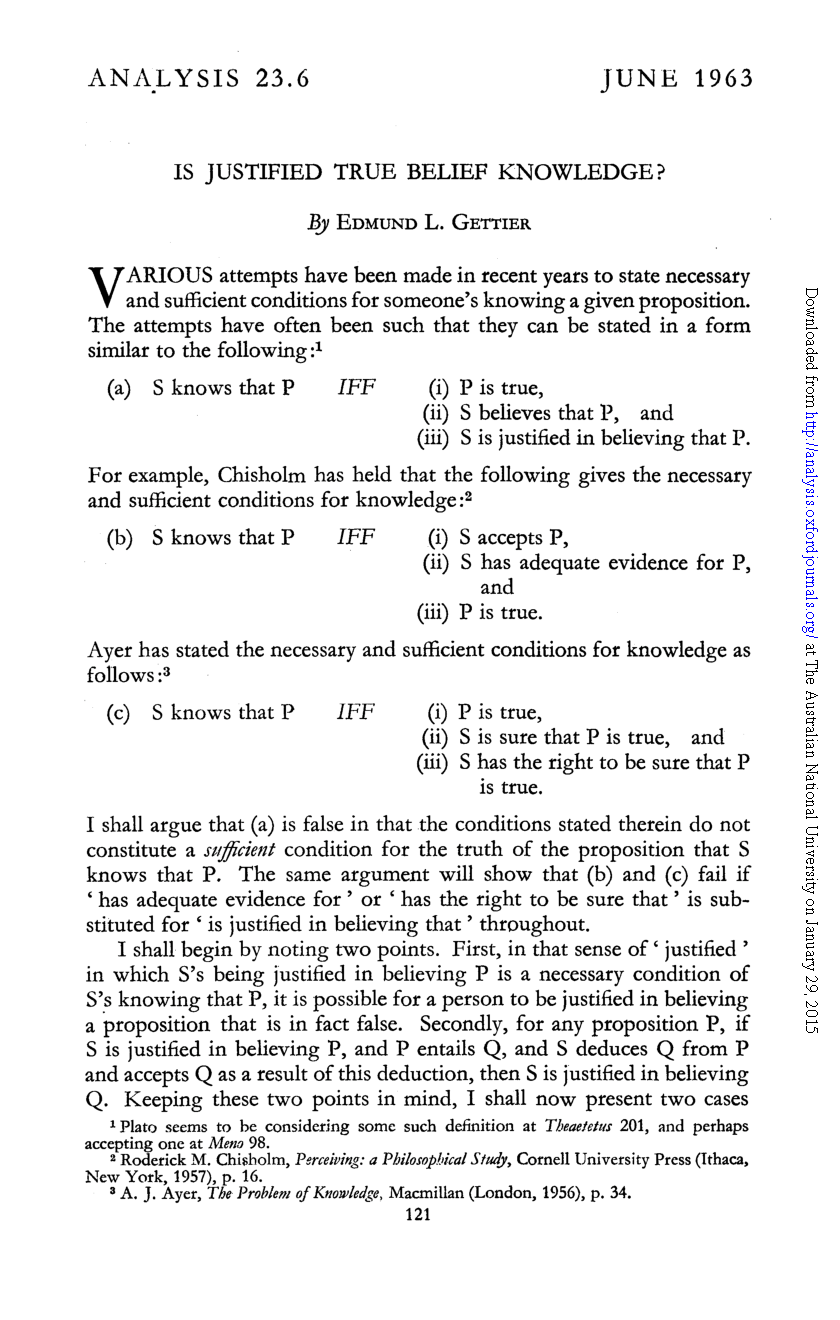
\includegraphics[width=0.5\linewidth]{figures/paper_gettier_1963.pdf}}\\
      \textcolor{gray}{Gettier (1963)}\\
      \frame{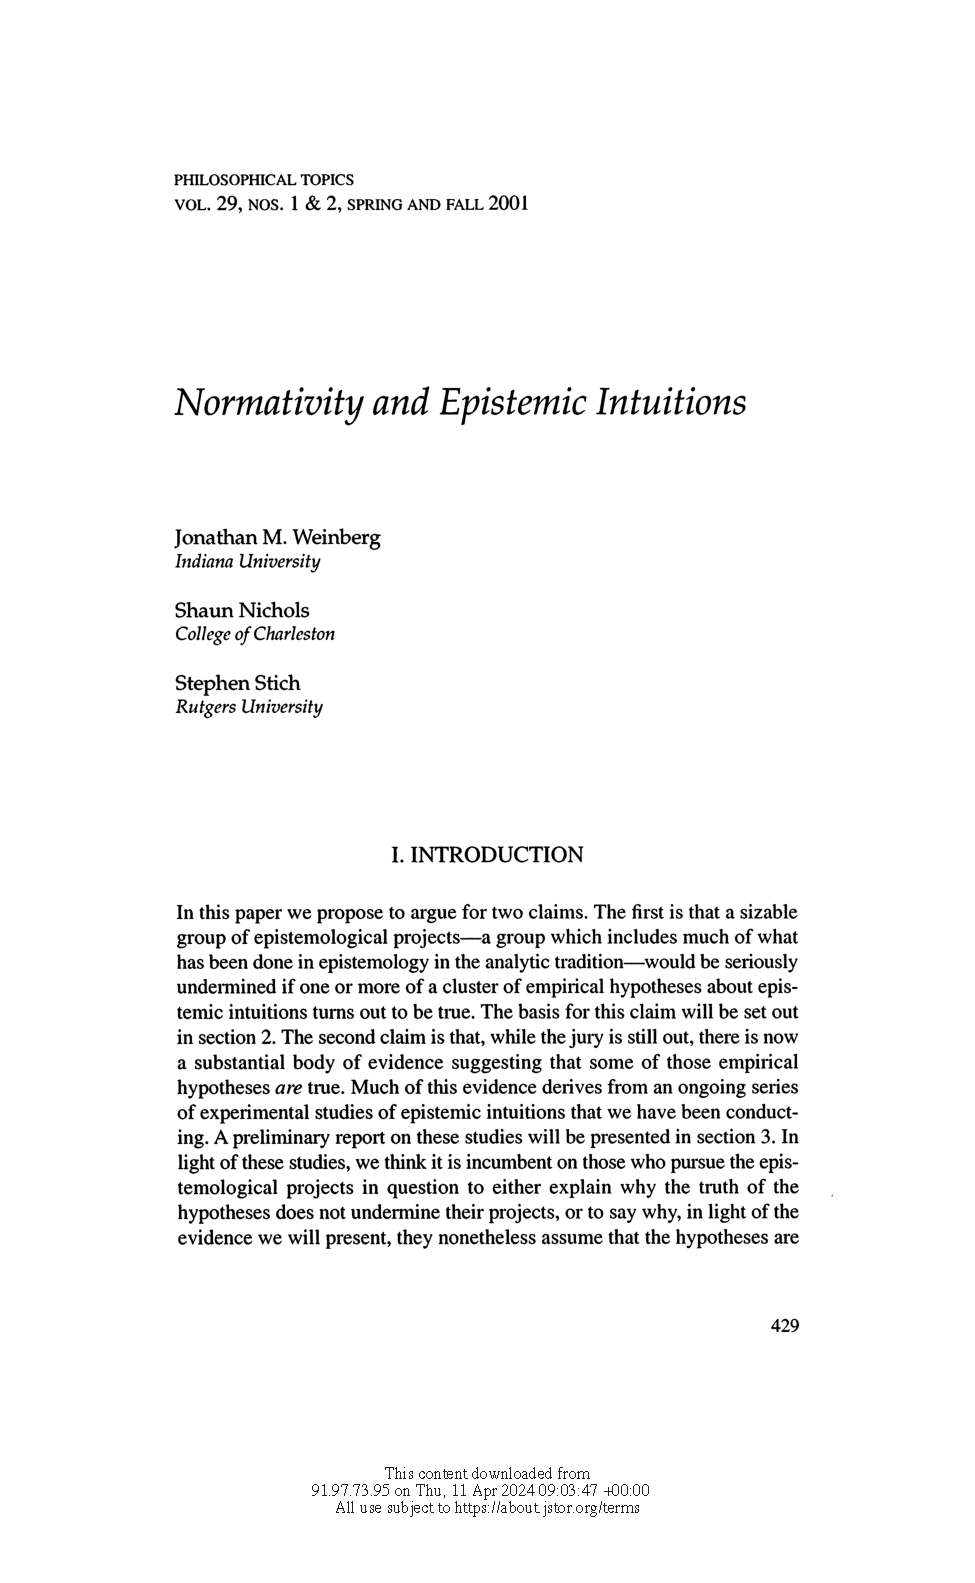
\includegraphics[width=0.5\linewidth]{figures/paper_weinberg_2001.pdf}}\\
      \textcolor{gray}{Weinberg, Nichols und Stich (2001)}
   \end{center}
\end{multicols}
\end{frame}


%%%%%%%%%%%%%%%%%%%%%%%%%
% FOLIE 6 – REPLIKATION %
%%%%%%%%%%%%%%%%%%%%%%%%%
\begin{frame}
\begin{overlayarea}{\textwidth}{0.81\paperheight}{
   \vspace*{11mm}
   \usebeamerfont{title}\textcolor{uolblue}
   {2\hspace*{1em}Replikationsstudie}
}
\end{overlayarea}
\end{frame}


%%%%%%%%%%%
% FOLIE 7 %
%%%%%%%%%%%
\begin{frame}{\vspace*{10mm}2\hspace*{1em}Replikationsstudie}
\textbf{Originalstudie}\\
\begin{center}
   \frame{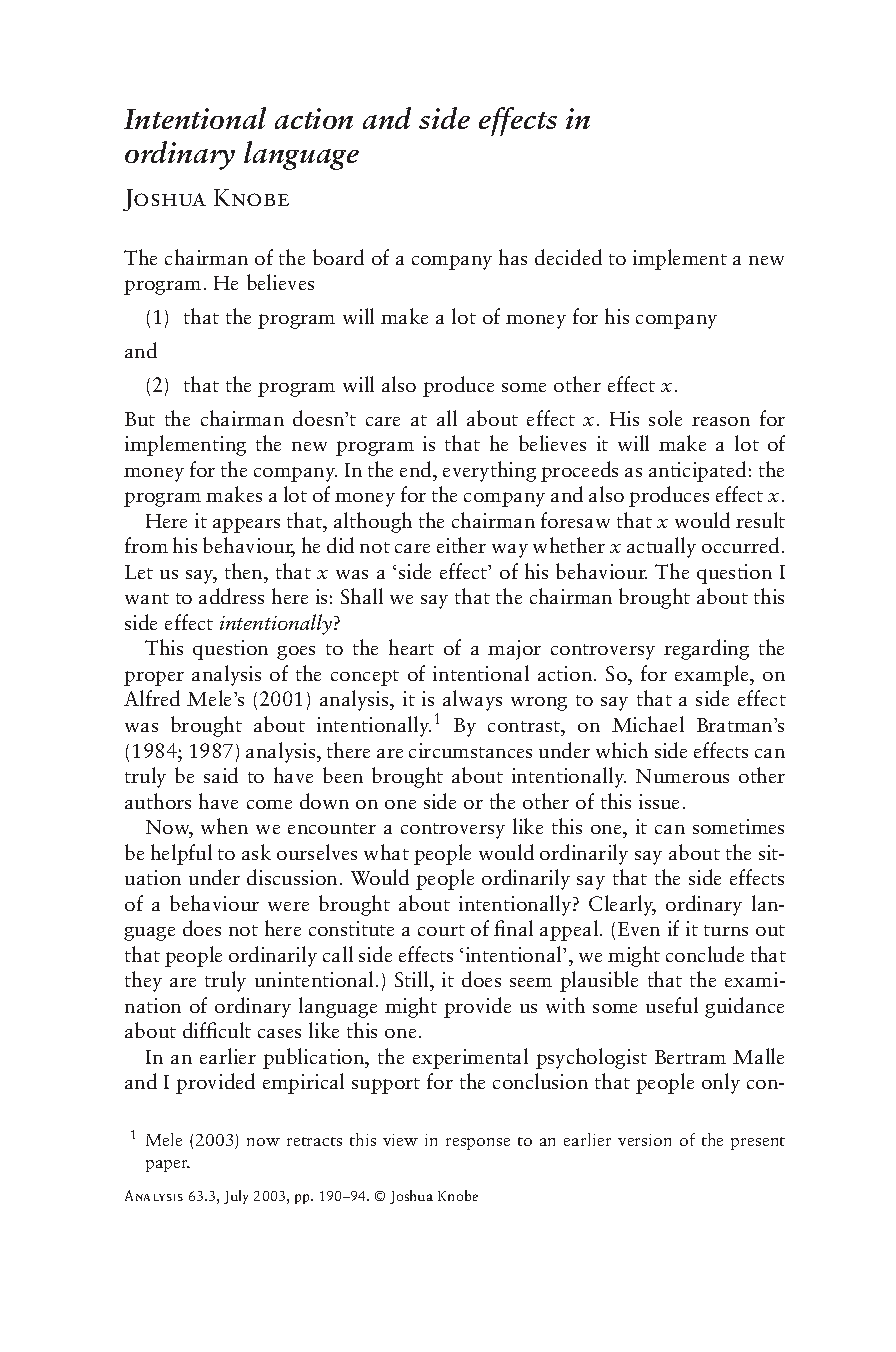
\includegraphics[width=0.25\linewidth]{figures/paper_knobe_2003.pdf}}\\
   \textcolor{gray}{Knobe (2003)}
\end{center}
\end{frame}


%%%%%%%%%%%
% FOLIE 8 %
%%%%%%%%%%%
\begin{frame}{\vspace*{10mm}2\hspace*{1em}Replikationsstudie}
\textbf{Problemstruktur}\\
\begin{center}
   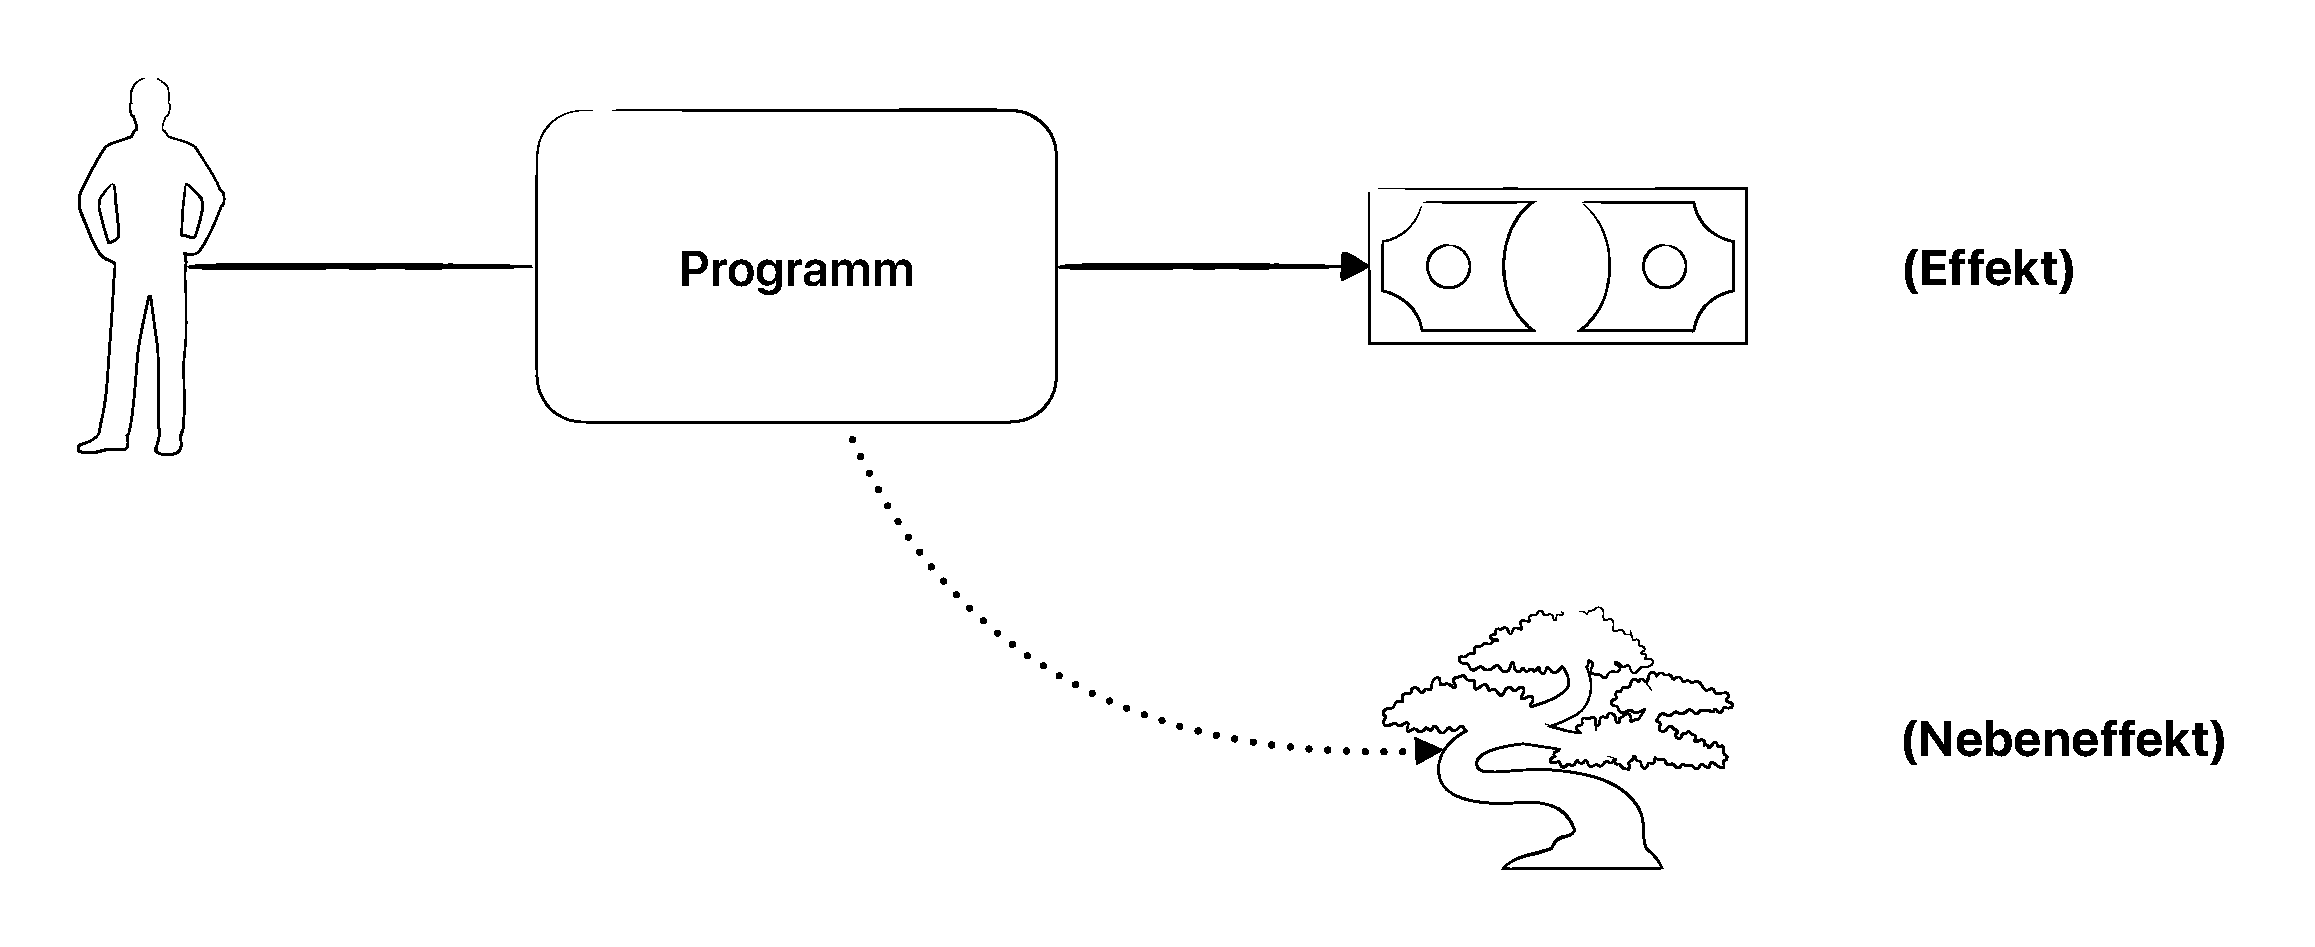
\includegraphics[width=0.75\linewidth]{figures/replication_knobe_structure.pdf}\\
\end{center}
\enquote{Shall we say that the chairman brought about this side effect \textit{intentionally}?}\\
\textcolor{gray}{(Knobe 2003, S. 190)}
\bigskip
\end{frame}


%%%%%%%%%%%
% FOLIE 9 %
%%%%%%%%%%%
\begin{frame}{\vspace*{10mm}2\hspace*{1em}Replikationsstudie}
\textbf{Studienaufbau}\\
\medskip
\begin{itemize}
   \item Zwei Varianten einer Vignette \textcolor{gray}{(Entscheidung schadet oder hilft der Umwelt)}
   \item Teilnehmer*innen sehen immer nur eine Variante der Vignette
   \item Im Anschluss zwei Fragen
   \begin{itemize}
      \item Wie tadelns- oder lobenswert ist die Person für ihre Entscheidung? \textcolor{gray}{(Skala von~0 bis~6)}
      \item Hat die Person den Nebeneffekt absichtlich herbeigeführt? \textcolor{gray}{(ja oder nein)}
   \end{itemize}
\end{itemize}
\end{frame}


%%%%%%%%%%%%
% FOLIE 10 %
%%%%%%%%%%%%
\begin{frame}{\vspace*{10mm}2\hspace*{1em}Replikationsstudie}
\textbf{Vignette}\\
\medskip
\enquote{The vice-president of a company went to the chairman of the board and said, \enquote{We are thinking of starting a new program. It will help us increase profits, but \textcolor{blue2}{[and]} it will also harm \textcolor{blue2}{[help]} the environment.}\\\vspace{0.5em}
The chairman of the board answered, \enquote{I don't care at all about harming \textcolor{blue2}{[helping]} the environment. I just want to make as much profit as I can. Let's start the new program.}\\\vspace{0.5em}
They started the new program. Sure enough, the environment was harmed \textcolor{blue2}{[helped]}.}\\
\textcolor{gray}{(Knobe 2003, S. 190)}
\bigskip

\textbf{Fragen}\\
\begin{itemize}
   \item \enquote{These subjects were then asked to determine how much blame the
chairman deserved for what he did (on a scale from 0 to 6)} \textcolor{gray}{(ebd., S. 191)}
   \item \enquote{These subjects were then asked [$\cdots$] to say whether they thought the chairman \textit{intentionally} harmed the environment} \textcolor{gray}{(ebd.)}
\end{itemize}
\end{frame}


%%%%%%%%%%%%%%%%%%%%%%%%%%%
% FOLIE 11 – BIBLIOGRAFIE %
%%%%%%%%%%%%%%%%%%%%%%%%%%%
\begin{frame}{\vspace*{10mm}Bibliografie}
\vspace*{-5mm}
{\footnotesize
\begin{itemize}[label=,leftmargin=2em,itemindent=-2em]
   \item Gettier, Edmund (1963): \enquote{Is Justified True Belief Knowledge?}, \textit{Analysis} 23 (6), S.~121--123.
   \item Knobe, Joshua (2003): \enquote{Intentional Action and Side Effects in Ordinary Language}, \textit{Analysis} 63 (3), S. 190--194.
   \item Weinberg, Jonathan, Shaun Nichols und Stephen Stich (2001): \enquote{Normativity and Epistemic Intuitions}, \textit{Philosophical Topics} 29 (1/2), S.~429--460.
\end{itemize}
}
\end{frame}


\end{document}
